\section{Evaluation on Synthetic Data}
\label{sec:evasim}

Evaluation on synthetic data is used to establish the benefit of the POPP and its variations over the FOPP in estimating the arrival rate $\lambda$ of a Poisson process. With synthetic data, sensor reliability can be controlled, and the true $\lambda$ and the true counts $c_i$ are known in advance for each sample. Here, an evaluation and a comparison of the POPP models to the FOPP model are conducted with two imaginary unreliable sensors and simulated datasets. The switching filter is chosen as a filter for all POPP models for this evaluation.

In each experiment, The sensor model (for the POPP and POPP-Beta models) and joint sensor model (for the C-POPP and POPP-Dirichlet models) is first built based on the sampled counts $c_1, \ldots, c_n$ from a Poisson process $P(c ; \lambda'=3)$ and the corresponding sensor readings $\protect\overrightarrow{s_1} \ldots \protect\overrightarrow{s_{n}}$. Then another set of counts $c_1, \ldots, c_{144}$ is sampled from the same process. These counts were then fed to simulated sensors that counted unreliably, producing sensor readings $\protect\overrightarrow{s_1} \ldots \protect\overrightarrow{s_{144}}$. A recursive update, then, takes place on $P(\lambda ; \overrightarrow{s_i})$ using the switching filter.

Two different sample sizes used to build the (joint) sensor model were chosen: a small number of samples, and a large number of samples. A small number of samples build an erroneous (joint) sensor model. In the POPP-Dirichlet and the POPP-Beta models, a small number of samples creates a loose Dirichlet and beta densities. Conversely, a large number of samples creates a low variance, and thus reliable, (joint) sensor model by tightening the Dirichlet prior of the POPP-Dirichlet model and the Beta prior of the POPP-Beta model. 120 samples were set for the small sample size, and 2880 samples were set for the large sample size.

Different correlations between two sensors were tested: positive correlation, negative correlation, and no correlation. These correlations are aimed to show the benefit of the C-POPP and POPP-Dirichlet models over any other model including the POPP and the POPP-Beta models. One should note that under the POPP and POPP-Beta models, sensors are assumed to be uncorrelated.  

\begin{figure}[t!]
	\centering
	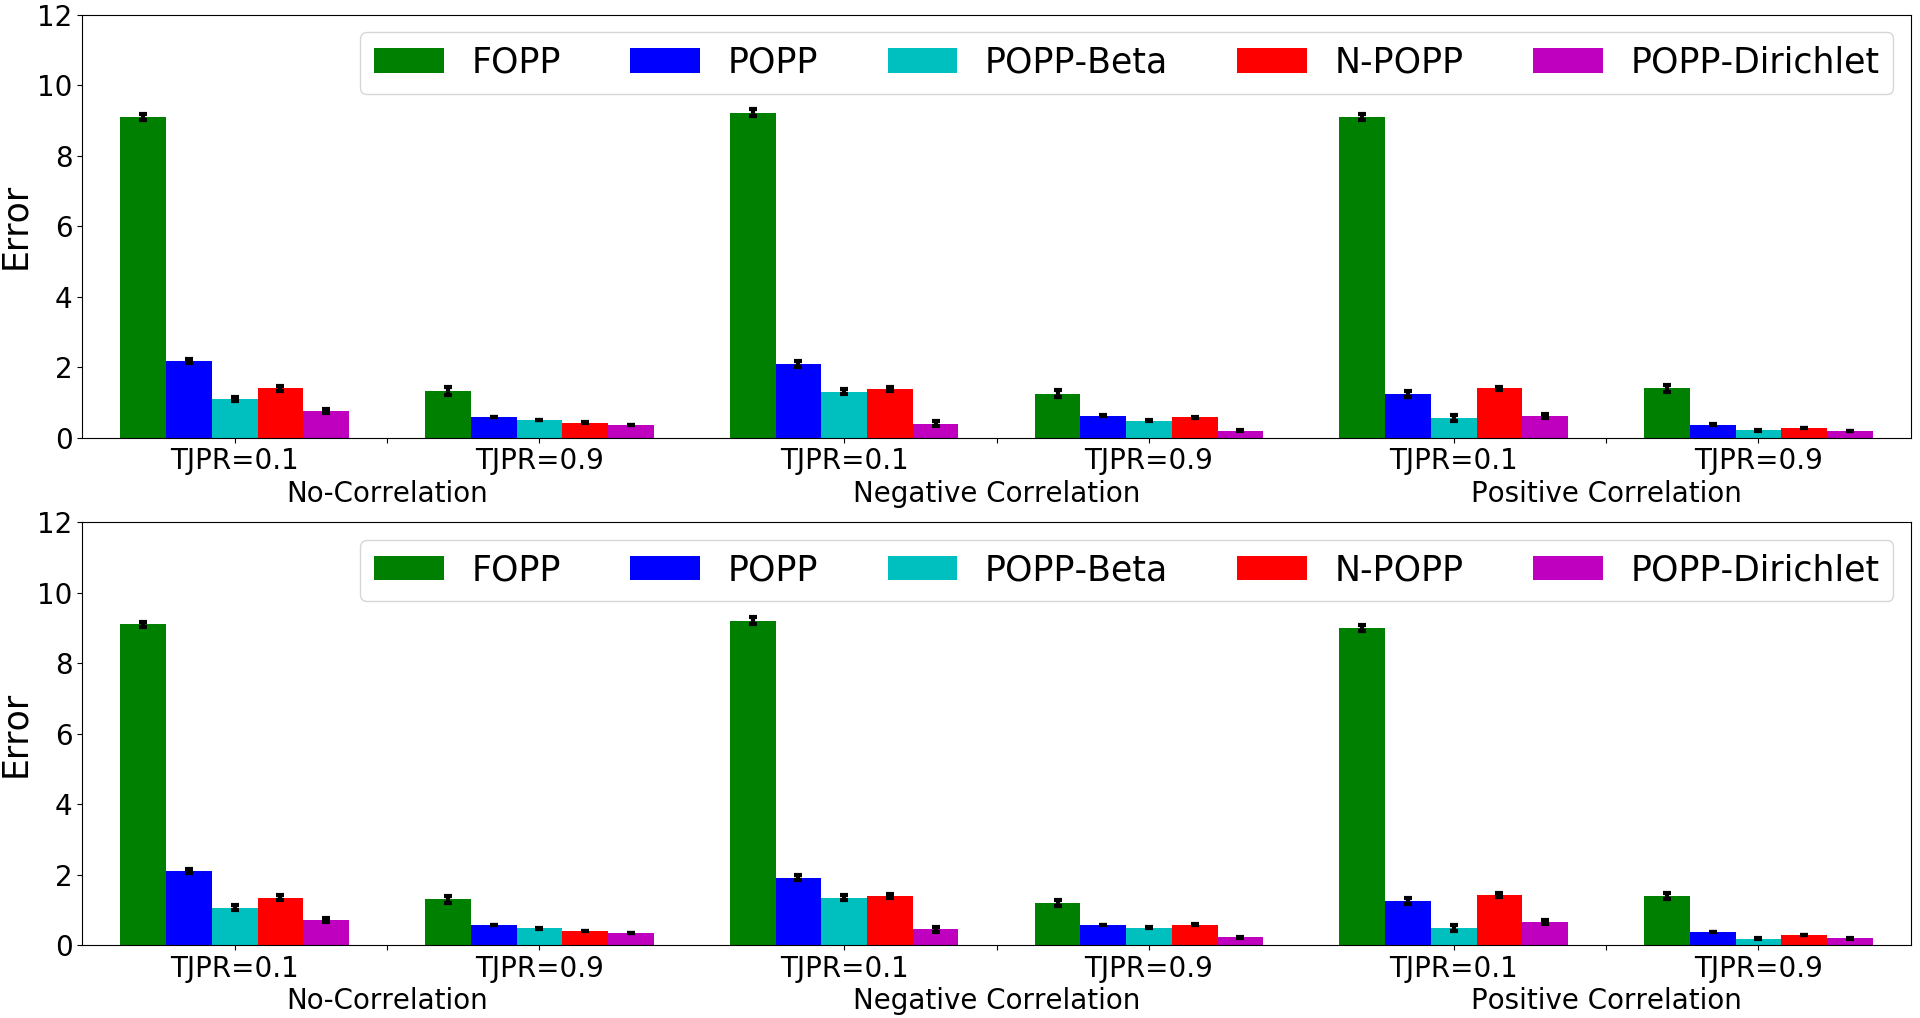
\includegraphics[width=0.5\textwidth]{./figures/tjpr_comparison_120.png}
    \caption{The RMSE of posterior estimates of $\lambda$ for the POPP-Dirichlet and other POPP models with 120 sample data used to build the (joint) sensor model with variation on $\mathcal{E^+}$. Each trial consisted of a stream of $\protect\overrightarrow{s_1} \ldots \protect\overrightarrow{s_{144}}$ samples to update $P(\lambda ; \protect\overrightarrow{s_i})$. Accuracies of MAP estimates are shown in the top panel, accuracies of expectation of the posterior in the bottom panel. Each data point is an average of 30 trials. Standard errors are shown.} 
	\label{fig:tjpr_comparison_120}
\end{figure}

\begin{figure}[t!]
	\centering
	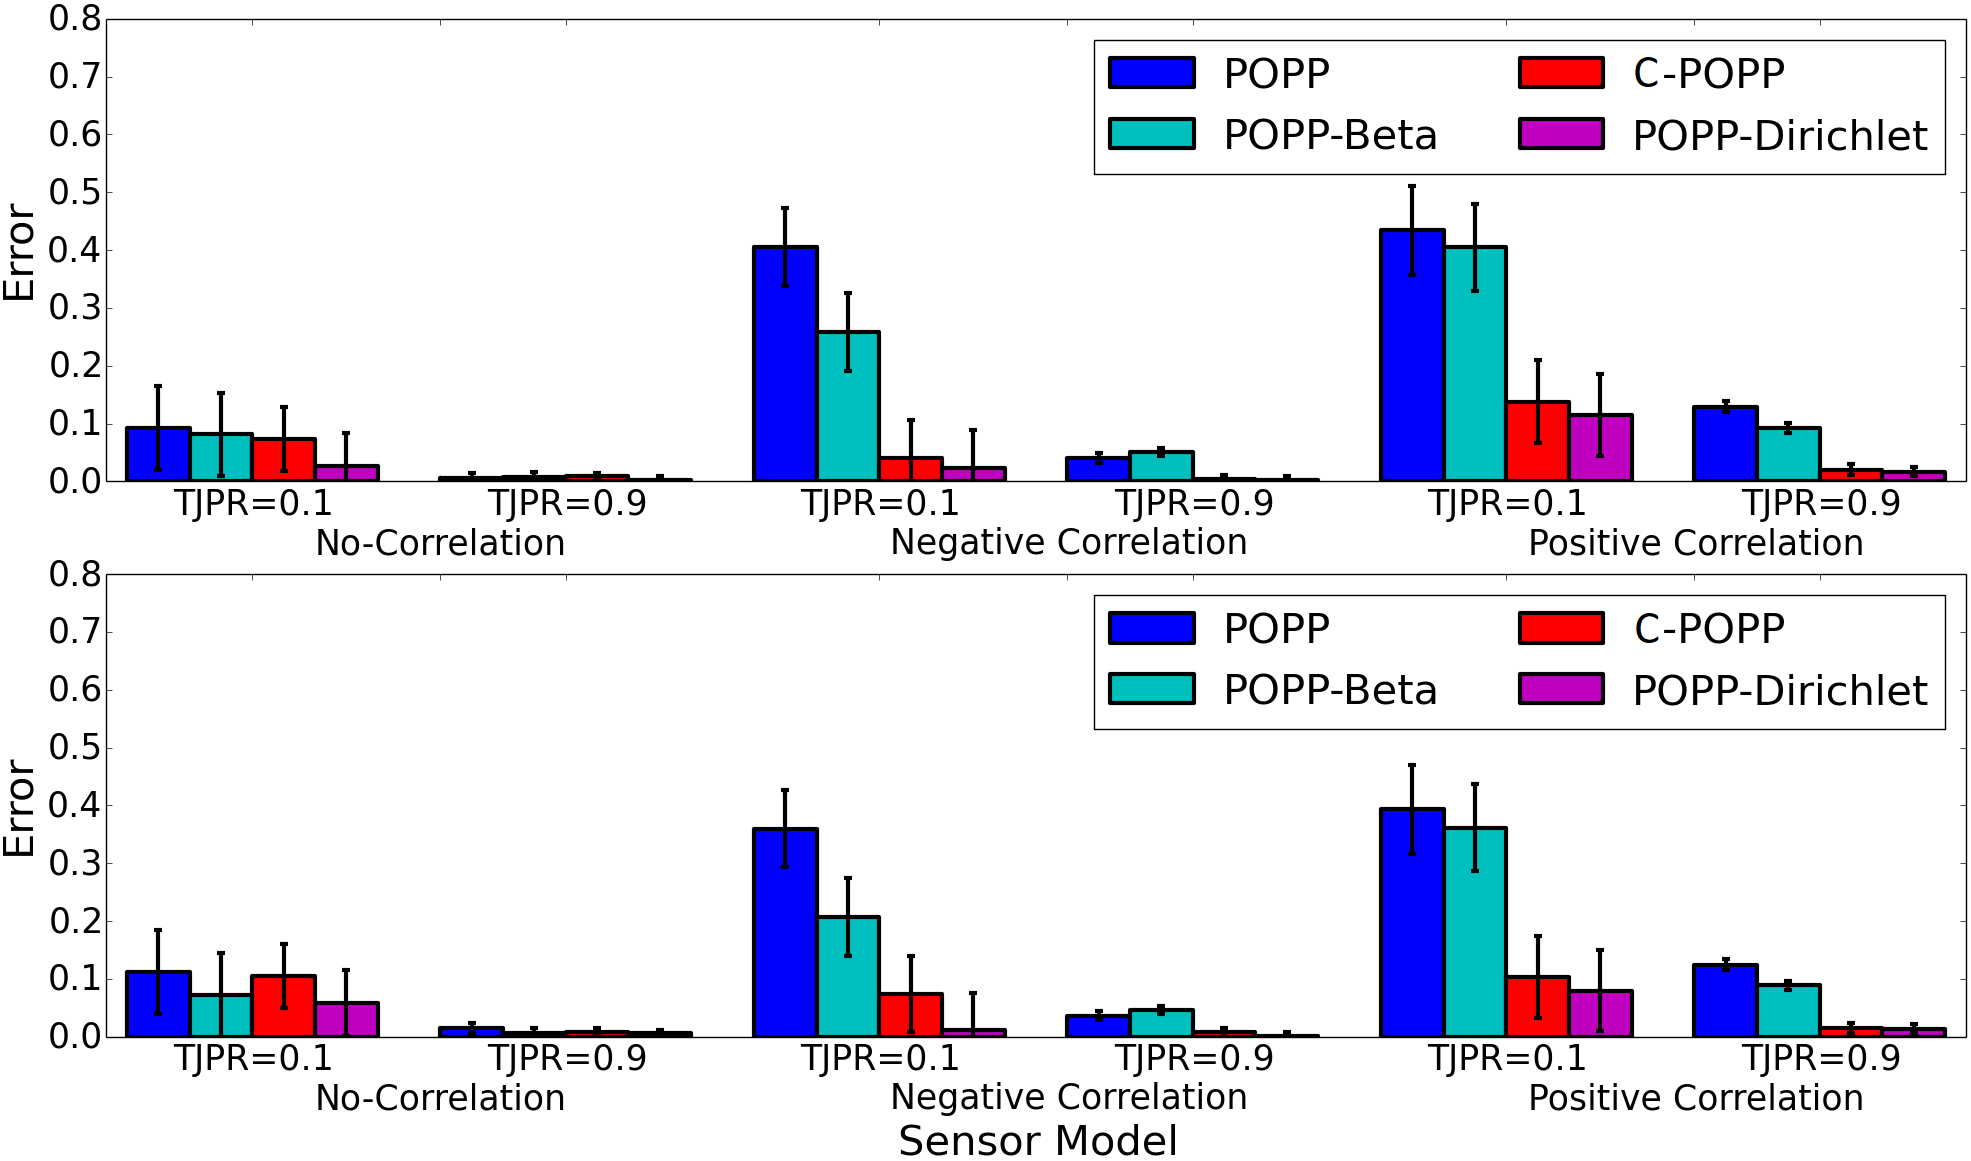
\includegraphics[width=0.5\textwidth]{./figures/tjpr_comparison_2880.png}
    \caption{The RMSE of posterior estimates of $\lambda$ for the POPP-Dirichlet and other POPP models with 2880 sample data used to build the (joint) sensor model with variation on $\mathcal{E^+}$. Each trial consisted of a stream of $\protect\overrightarrow{s_1} \ldots \protect\overrightarrow{s_{144}}$ samples to update $P(\lambda ; \protect\overrightarrow{s_i})$. Accuracies of MAP estimates are in the top panel, accuracies of expectation of the posterior in the bottom panel. Each data point is an average of 30 trials. Standard errors are shown.} 
	\label{fig:tjpr_comparison_2880}
\end{figure}

For each correlation type, a further variation to different levels of sensor unreliability was considered. First, two variations were made to the true joint positive rate $\mathcal{E^+}$ (TJPR), while fixing the true joint negative rate $\mathcal{E^-}$ (TJNR) on each type of correlation. This includes:
\begin{itemize}
    \item $P_{jnt}(d_{1k}=1, d_{2k}=1 ; e_k=1) = 0.1, P_{jnt}(d_{1k}=0, d_{2k}=0 ; e_k=1) = 0.9$ ($\mathcal{E^+}$ with low positive correlation);
    \item $P_{jnt}(d_{1k}=1, d_{2k}=1 ; e_k=1) = 0.9, P_{jnt}(d_{1k}=0, d_{2k}=0 ; e_k=1) = 0.1$ ($\mathcal{E^+}$ with high positive correlation);
    \item $P_{jnt}(d_{1k}=1, d_{2k}=0 ; e_k=1) = 0.05, P_{jnt}(d_{1k}=0, d_{2k}=1 ; e_k=1) = 0.05, P_{jnt}(d_{1k}=0, d_{2k}=0 ; e_k=1) = 0.9$ ($\mathcal{E^+}$ with low negative correlation);
    \item $P_{jnt}(d_{1k}=1, d_{2k}=0 ; e_k=1) = 0.45, P_{jnt}(d_{1k}=0, d_{2k}=1 ; e_k=1) = 0.45, P_{jnt}(d_{1k}=0, d_{2k}=0 ; e_k=1) = 0.1$ ($\mathcal{E^+}$ with high negative correlation);
    \item $P_{jnt}(d_{1k}=1, d_{2k}=0 ; e_k=1) = 0.033, P_{jnt}(d_{1k}=0, d_{2k}=1 ; e_k=1) = 0.033, P_{jnt}(d_{1k}=1, d_{2k}=1 ; e_k=1) = 0.033, P_{jnt}(d_{1k}=0, d_{2k}=0 ; e_k=1) = 0.901$ ($\mathcal{E^+}$ with no correlation -- Similar to a sensor model with TPR = 0.066);
    \item $P_{jnt}(d_{1k}=1, d_{2k}=0 ; e_k=1) = 0.3, P_{jnt}(d_{1k}=0, d_{2k}=1 ; e_k=1) = 0.3, P_{jnt}(d_{1k}=1, d_{2k}=1 ; e_k=1) = 0.3, P_{jnt}(d_{1k}=0, d_{2k}=0 ; e_k=1) = 0.1$ ($\mathcal{E^+}$ with no correlation -- Similar to a sensor model with TPR = 0.6).
\end{itemize}

Second, two variations to the true joint negative rate $\mathcal{E^-}$ (TJNR), while fixing the true joint positive rate $\mathcal{E^+}$ (TJPR) on each type of correlation. This includes: 
\begin{itemize}
    \item $P_{jnt}(d_{1k}=1, d_{2k}=1 ; e_k=0) = 0.1, P_{jnt}(d_{1k}=0, d_{2k}=0 ; e_k=0) = 0.9$ ($\mathcal{E^-}$ with low positive correlation);
    \item $P_{jnt}(d_{1k}=1, d_{2k}=1 ; e_k=0) = 0.9, P_{jnt}(d_{1k}=0, d_{2k}=0 ; e_k=0) = 0.1$ ($\mathcal{E^-}$ with high positive correlation);
    \item $P_{jnt}(d_{1k}=1, d_{2k}=0 ; e_k=0) = 0.05, P_{jnt}(d_{1k}=0, d_{2k}=1 ; e_k=0) = 0.05, P_{jnt}(d_{1k}=0, d_{2k}=0 ; e_k=0) = 0.9$ ($\mathcal{E^-}$ with low negative correlation);
    \item $P_{jnt}(d_{1k}=1, d_{2k}=0 ; e_k=0) = 0.45, P_{jnt}(d_{1k}=0, d_{2k}=1 ; e_k=0) = 0.45, P_{jnt}(d_{1k}=0, d_{2k}=0 ; e_k=0) = 0.1$ ($\mathcal{E^-}$ with high negative correlation);
    \item $P_{jnt}(d_{1k}=1, d_{2k}=0 ; e_k=0) = 0.033, P_{jnt}(d_{1k}=0, d_{2k}=1 ; e_k=0) = 0.033, P_{jnt}(d_{1k}=1, d_{2k}=1 ; e_k=0) = 0.033, P_{jnt}(d_{1k}=0, d_{2k}=0 ; e_k=1) = 0.901$ ($\mathcal{E^-}$ with no correlation -- Similar to a sensor model with low TNR);
    \item $P_{jnt}(d_{1k}=1, d_{2k}=0 ; e_k=0) = 0.3, P_{jnt}(d_{1k}=0, d_{2k}=1 ; e_k=0) = 0.3, P_{jnt}(d_{1k}=1, d_{2k}=1 ; e_k=0) = 0.3, P_{jnt}(d_{1k}=0, d_{2k}=0 ; e_k=1) = 0.1$ ($\mathcal{E^-}$ with no correlation -- Similar to a sensor model with moderate TNR).
\end{itemize}

\begin{figure}[t!]
	\centering
	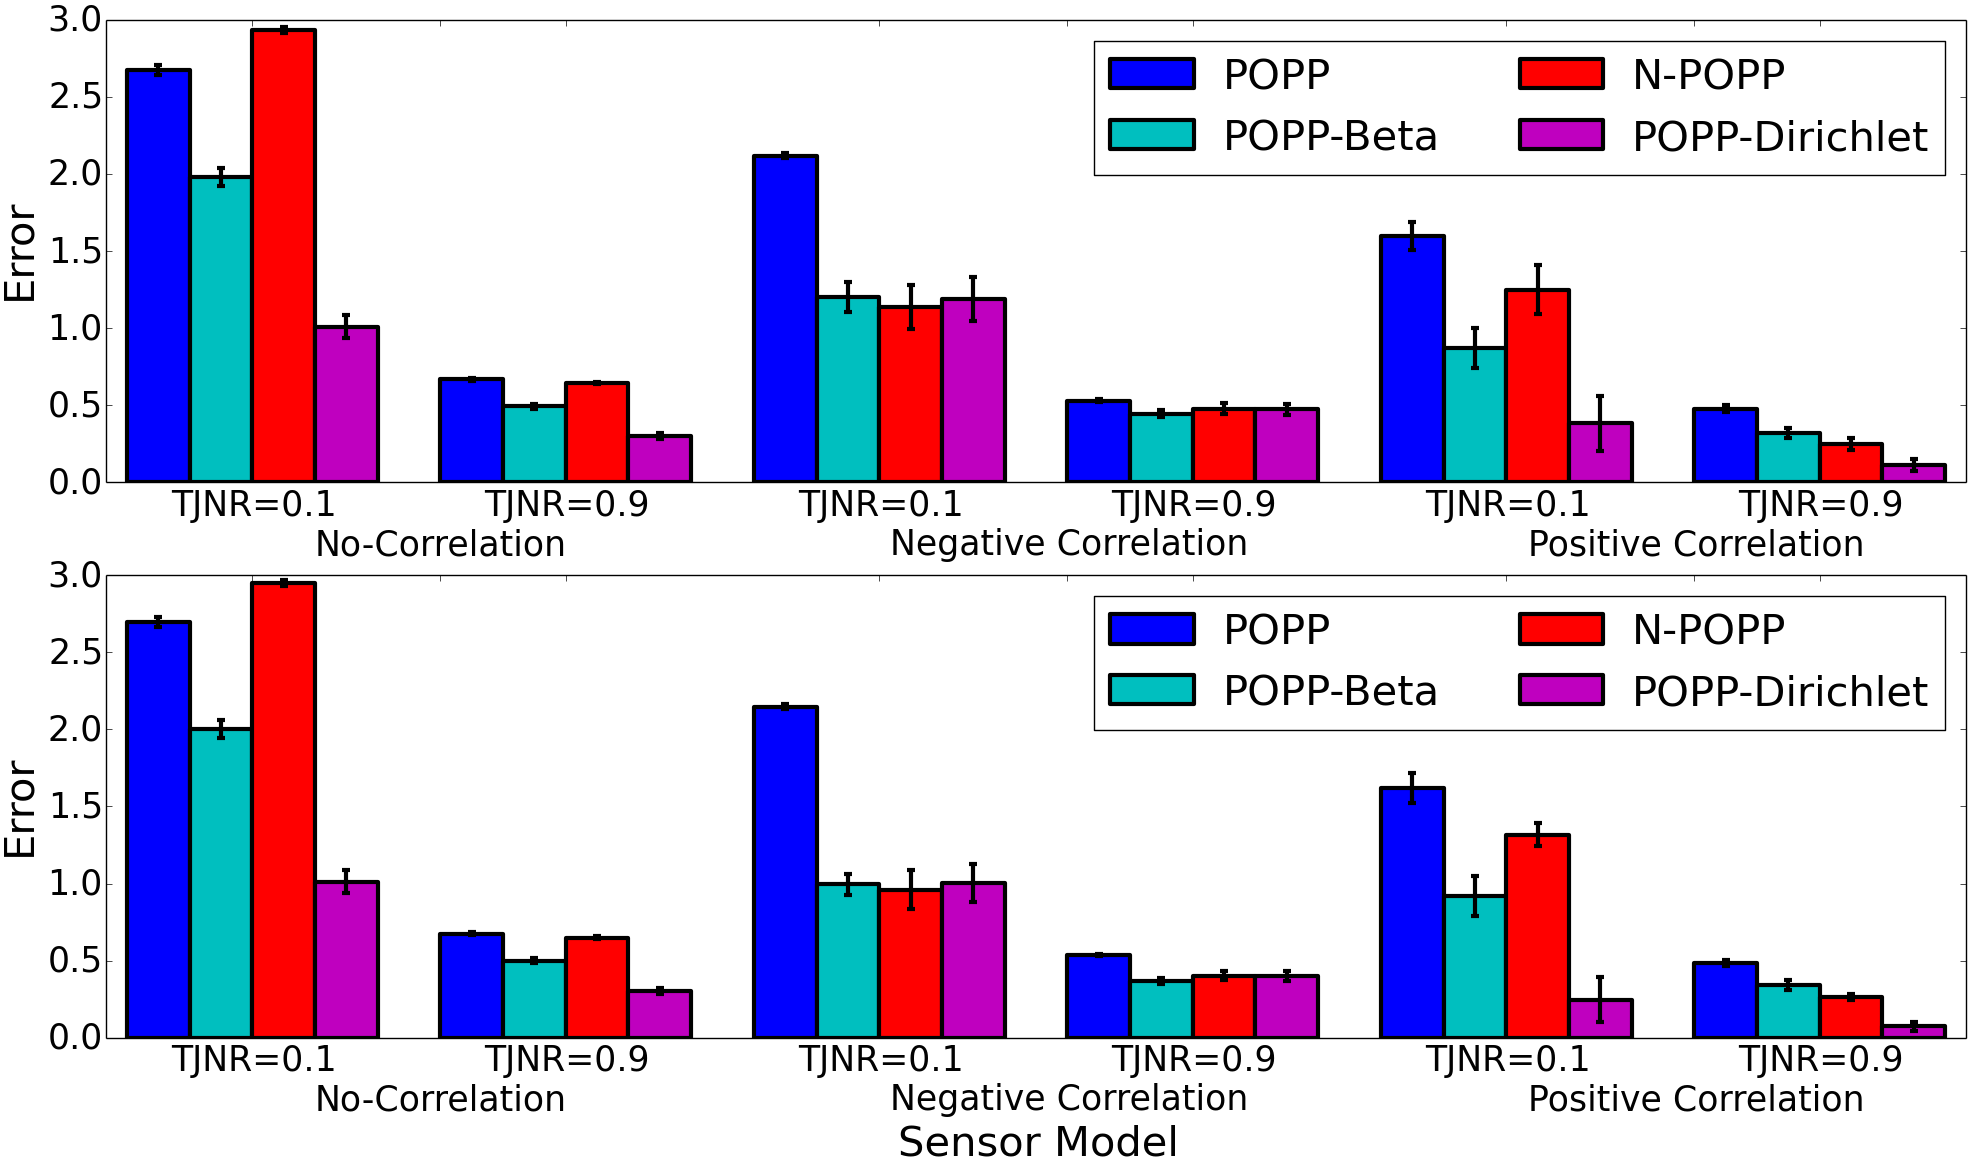
\includegraphics[width=0.5\textwidth]{./figures/tjnr_comparison_120.png}
    \caption{The RMSE of posterior estimates of $\lambda$ for the POPP-Dirichlet and other POPP models with 120 sample data used to build the (joint) sensor model with variation in $\mathcal{E^-}$. Each trial consisted of a stream of $\protect\overrightarrow{s_1} \ldots \protect\overrightarrow{s_{144}}$ samples to update $P(\lambda ; \protect\overrightarrow{s_i})$. Accuracies of MAP estimates are  in the top panel, accuracies of the expectation of the posterior in the bottom panel. Each data point is an average of 30 trials. Standard errors are shown.} 
	\label{fig:tjnr_comparison_120}
\end{figure}

\begin{figure}[t!]
	\centering
	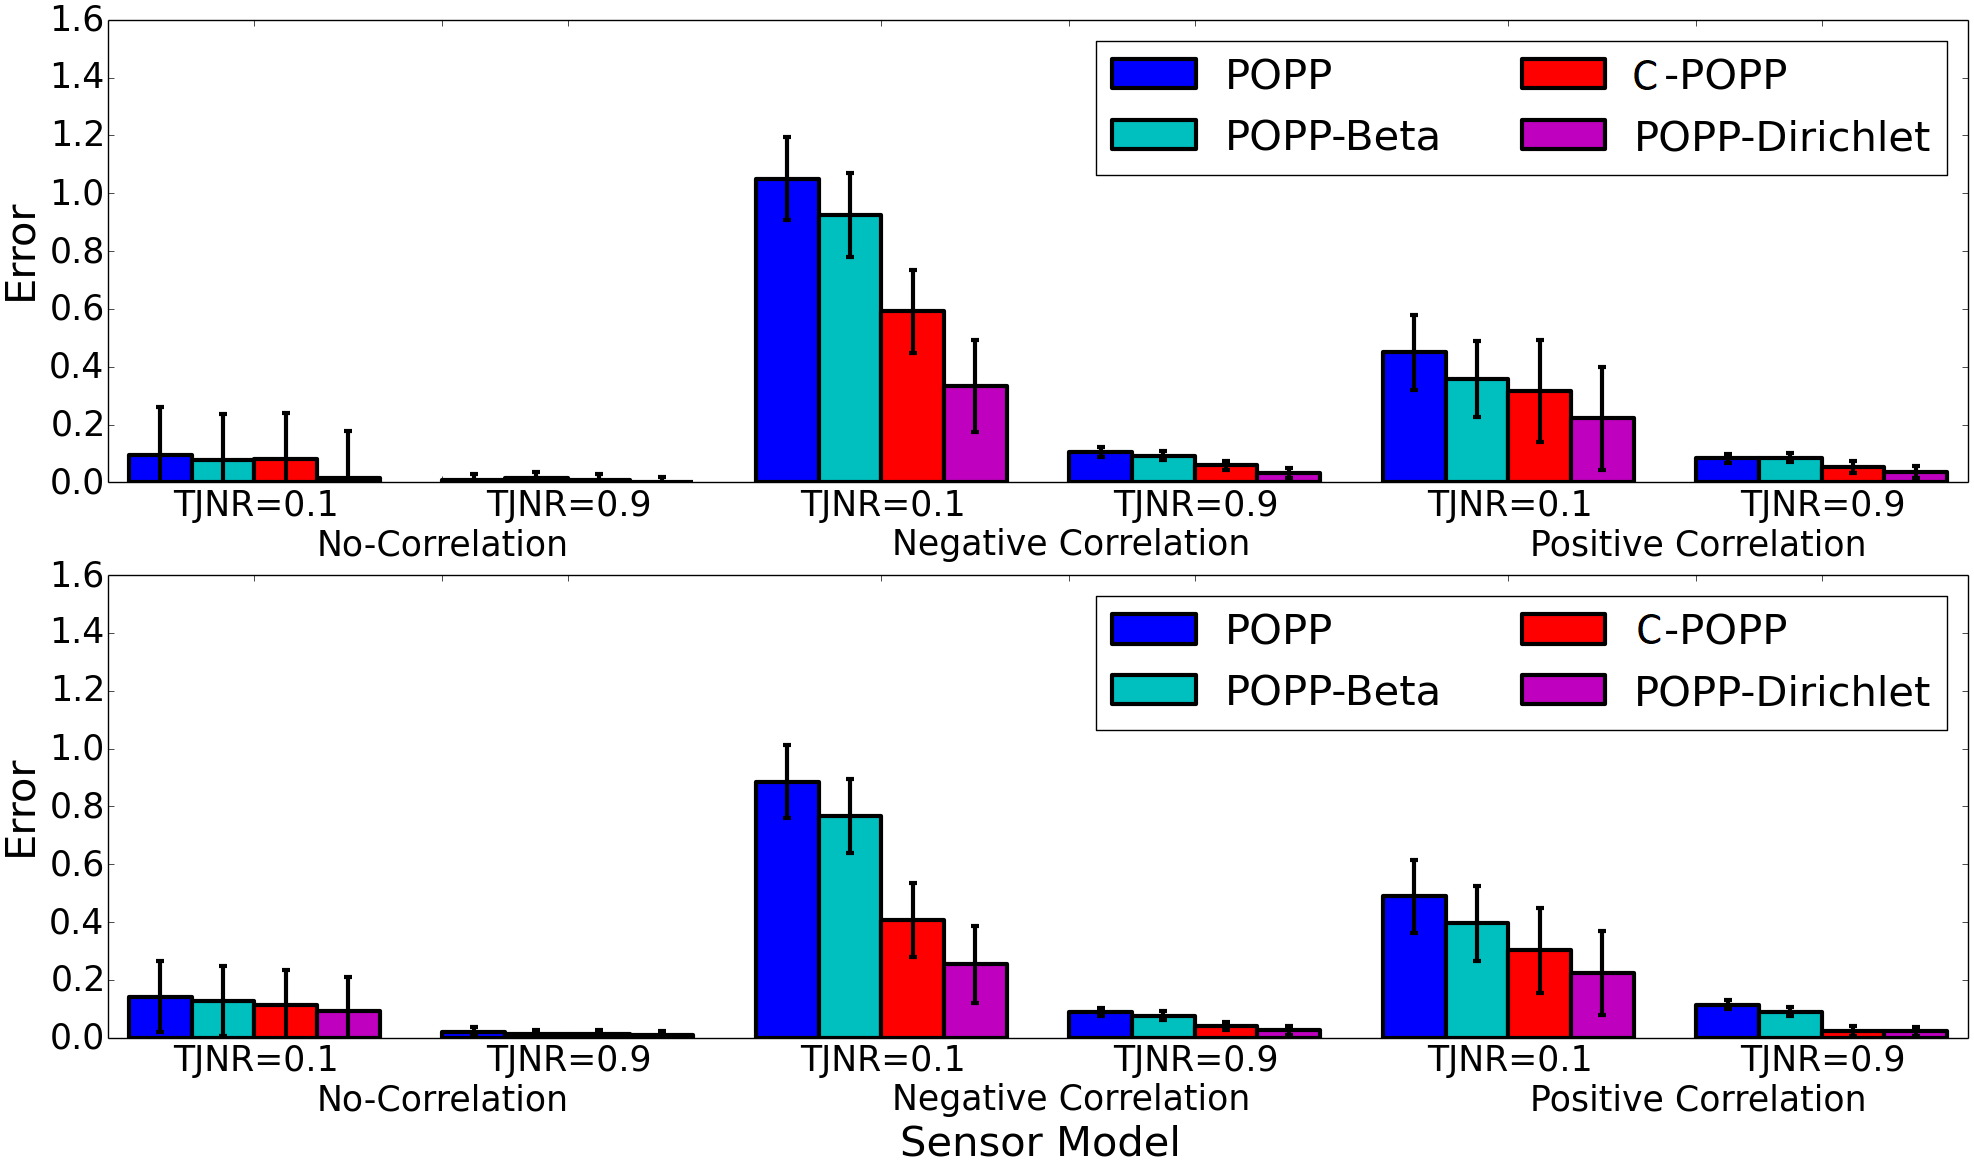
\includegraphics[width=0.5\textwidth]{./figures/tjnr_comparison_2880.png}
    \caption{The RMSE of posterior estimates of $\lambda$ for the POPP-Dirichlet and other POPP models with 2880 sample data used to build the (joint) sensor model with variation in $\mathcal{E^-}$. Each trial consisted of a stream of $\protect\overrightarrow{s_1} \ldots \protect\overrightarrow{s_{144}}$ samples to update $P(\lambda ; \protect\overrightarrow{s_i})$. Accuracies of MAP estimates are in the top panel, accuracies of the expectation of the posterior in the bottom panel. Each data point is an average of 30 trials. Standard errors are shown.} 
	\label{fig:tjnr_comparison_2880}
\end{figure}

The performance of all POPP models and the FOPP model were also assessed by comparing the Jensen-Shannon distance. Jensen-Shannon distance is a unit of measurement used in Jensen-Shannon divergence. The Jensen-Shannon divergence is a method of measuring the similarity between two probability distributions. Unlike KL-divergence, Jensen-Shannon divergence is a symmetrized divergence where $D_{JS}(P \parallel Q)$ is equal to $D_{JS}(Q \parallel P)$.

\begin{figure}[t!]
	\centering
	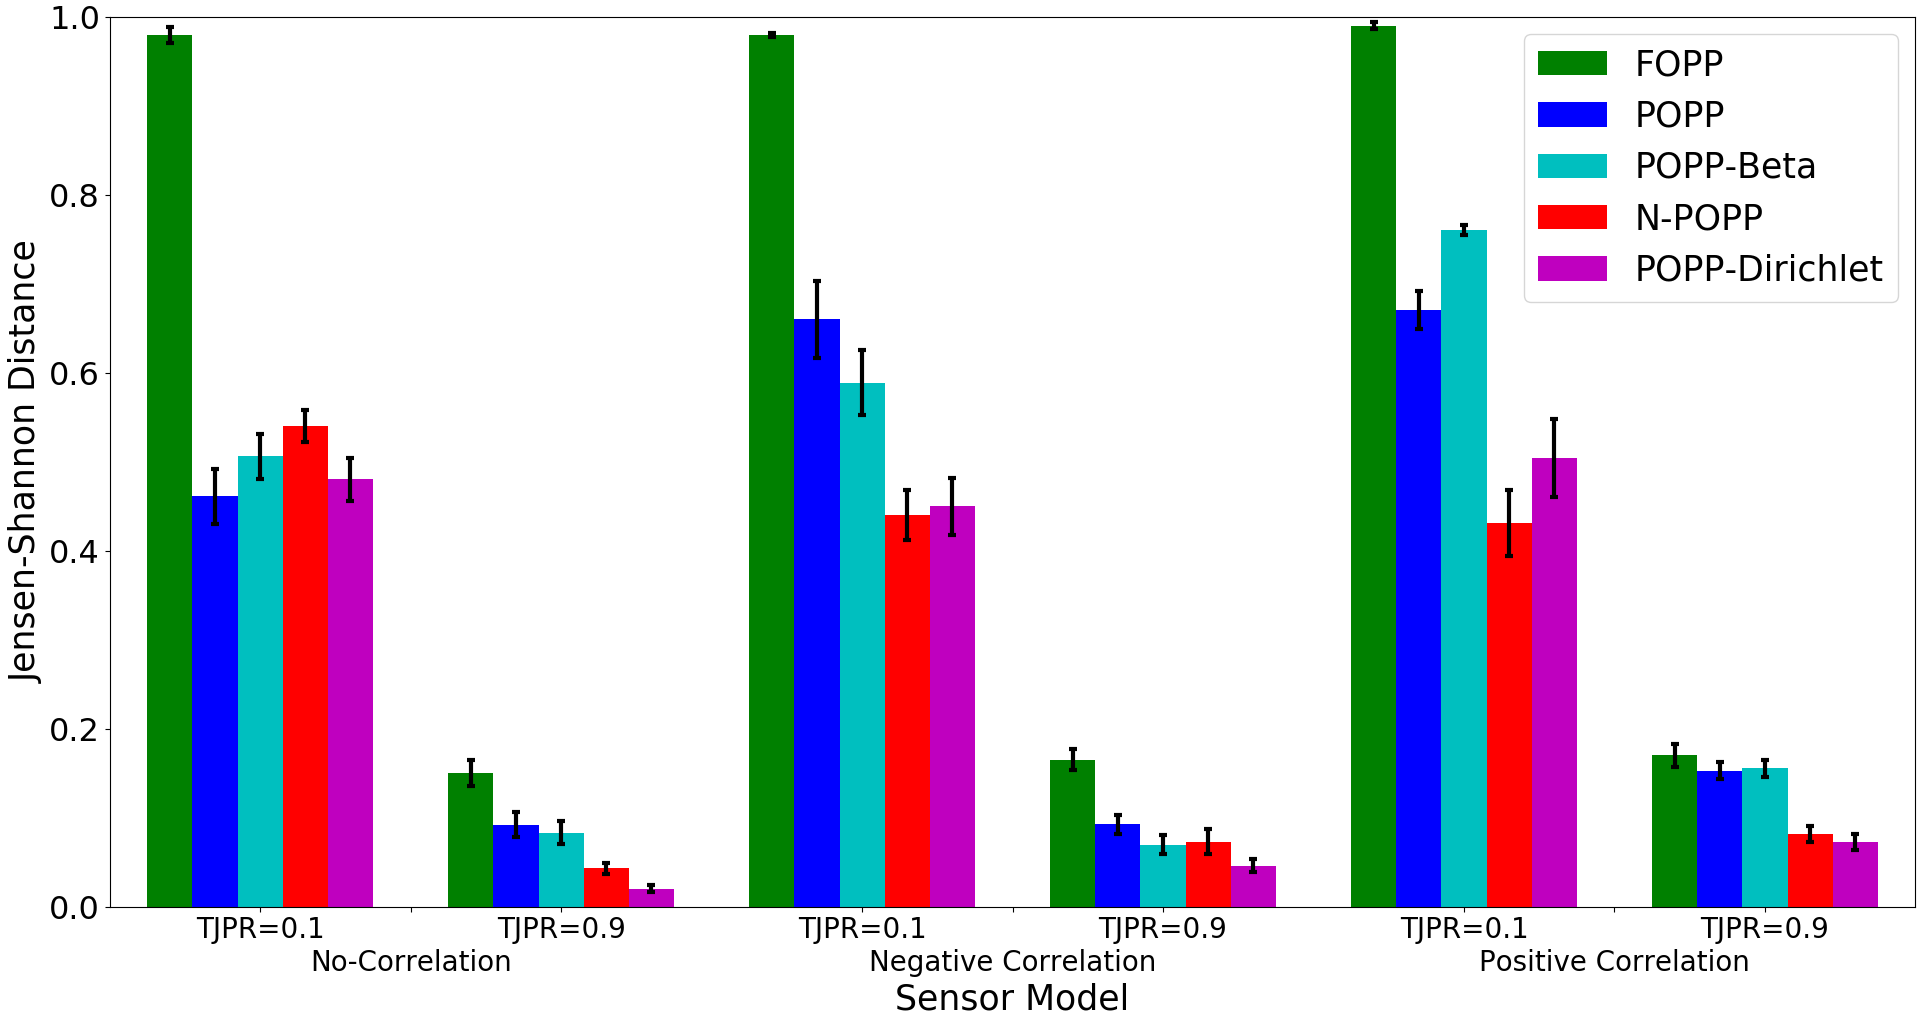
\includegraphics[width=0.5\textwidth]{./figures/tjpr_comparison_120_kl.png}
	\caption{The Jensen-Shannon distance of posterior estimates of $\lambda$ for the POPP-Dirichlet and other POPP models with 120 sample data used to build the (joint) sensor model with variation on $\mathcal{E^+}$. Each trial consisted of a stream of $\protect\overrightarrow{s_1} \ldots \protect\overrightarrow{s_{144}}$ samples to update $P_G(\lambda \mid \protect\overrightarrow{s_i})$. Each data point is an average of 30 trials. Standard errors are shown.} 
	\label{fig:tjpr_comparison_120_kl}
\end{figure}

\begin{figure}[t!]
	\centering
	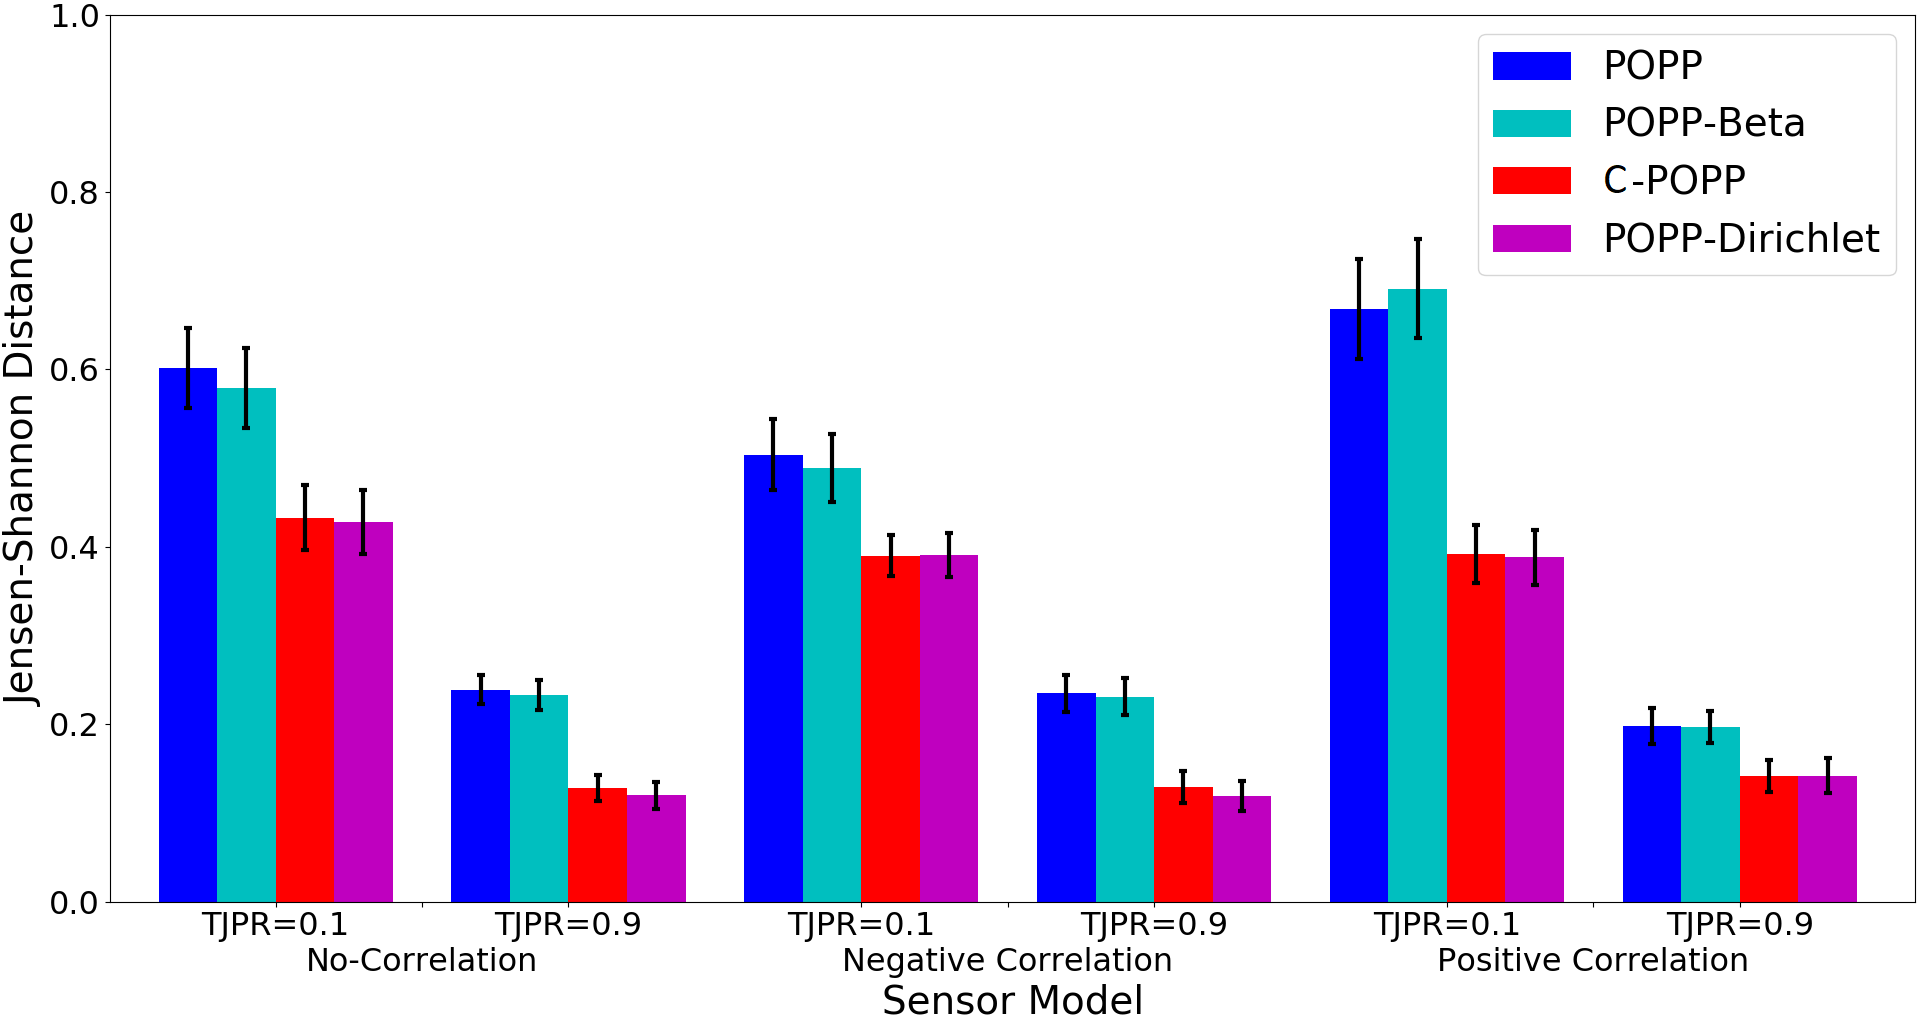
\includegraphics[width=0.5\textwidth]{./figures/tjpr_comparison_2880_kl.png}
	\caption{The Jensen-Shannon distance of posterior estimates of $\lambda$ for the POPP-Dirichlet and other POPP models with 2880 sample data used to build the (joint) sensor model with variation on $\mathcal{E^+}$. Each trial consisted of a stream of $\protect\overrightarrow{s_1} \ldots \protect\overrightarrow{s_{144}}$ samples to update $P_G(\lambda \mid \protect\overrightarrow{s_i})$. Each data point is an average of 30 trials. Standard errors are shown.} 
	\label{fig:tpjr_comparison_2880_kl}
\end{figure}

\begin{figure}[t!]
	\centering
	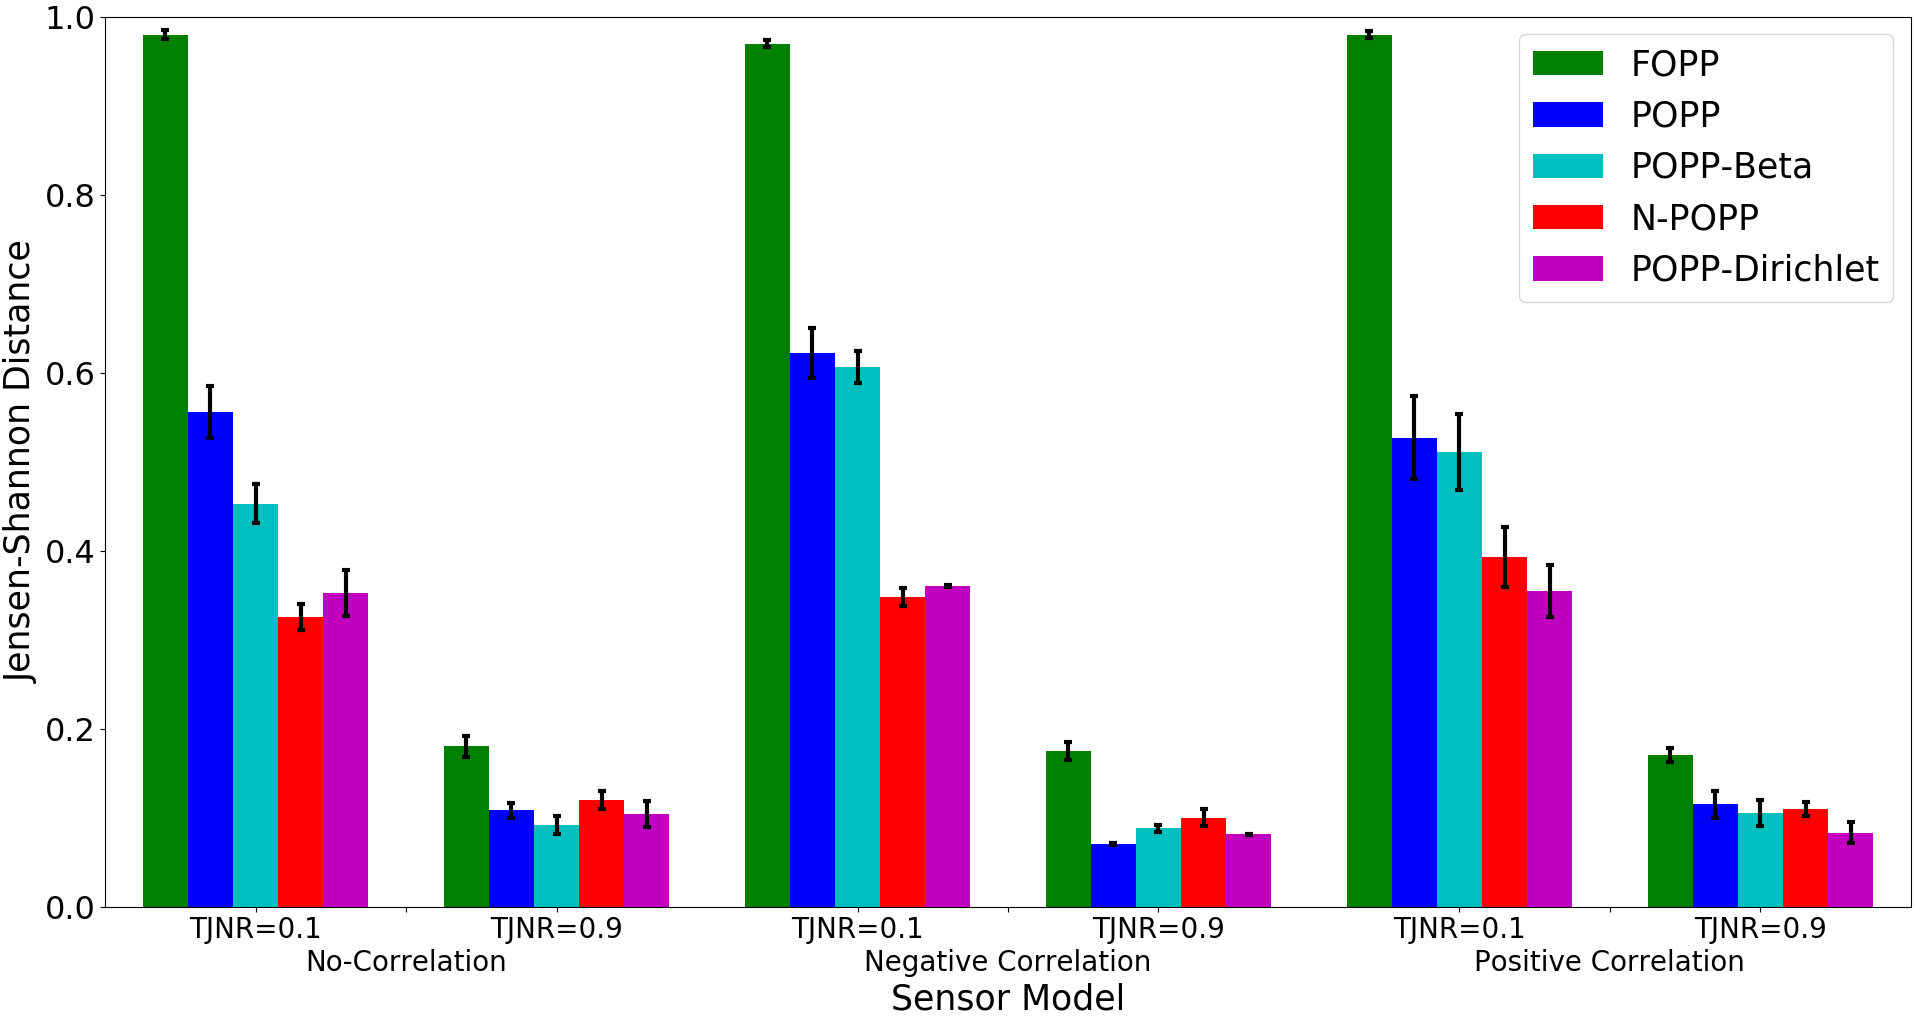
\includegraphics[width=0.5\textwidth]{./figures/tjnr_comparison_120_kl.png}
	\caption{The Jensen-Shannon distance of posterior estimates of $\lambda$ for the POPP-Dirichlet and other POPP models with 120 sample data used to build the (joint) sensor model with variation on $\mathcal{E^-}$. Each trial consisted of a stream of $\protect\overrightarrow{s_1} \ldots \protect\overrightarrow{s_{144}}$ samples to update $P_G(\lambda \mid \protect\overrightarrow{s_i})$. Each data point is an average of 30 trials. Standard errors are shown.} 
	\label{fig:tjnr_comparison_120_kl}
\end{figure}

\begin{figure}[t!]
	\centering
	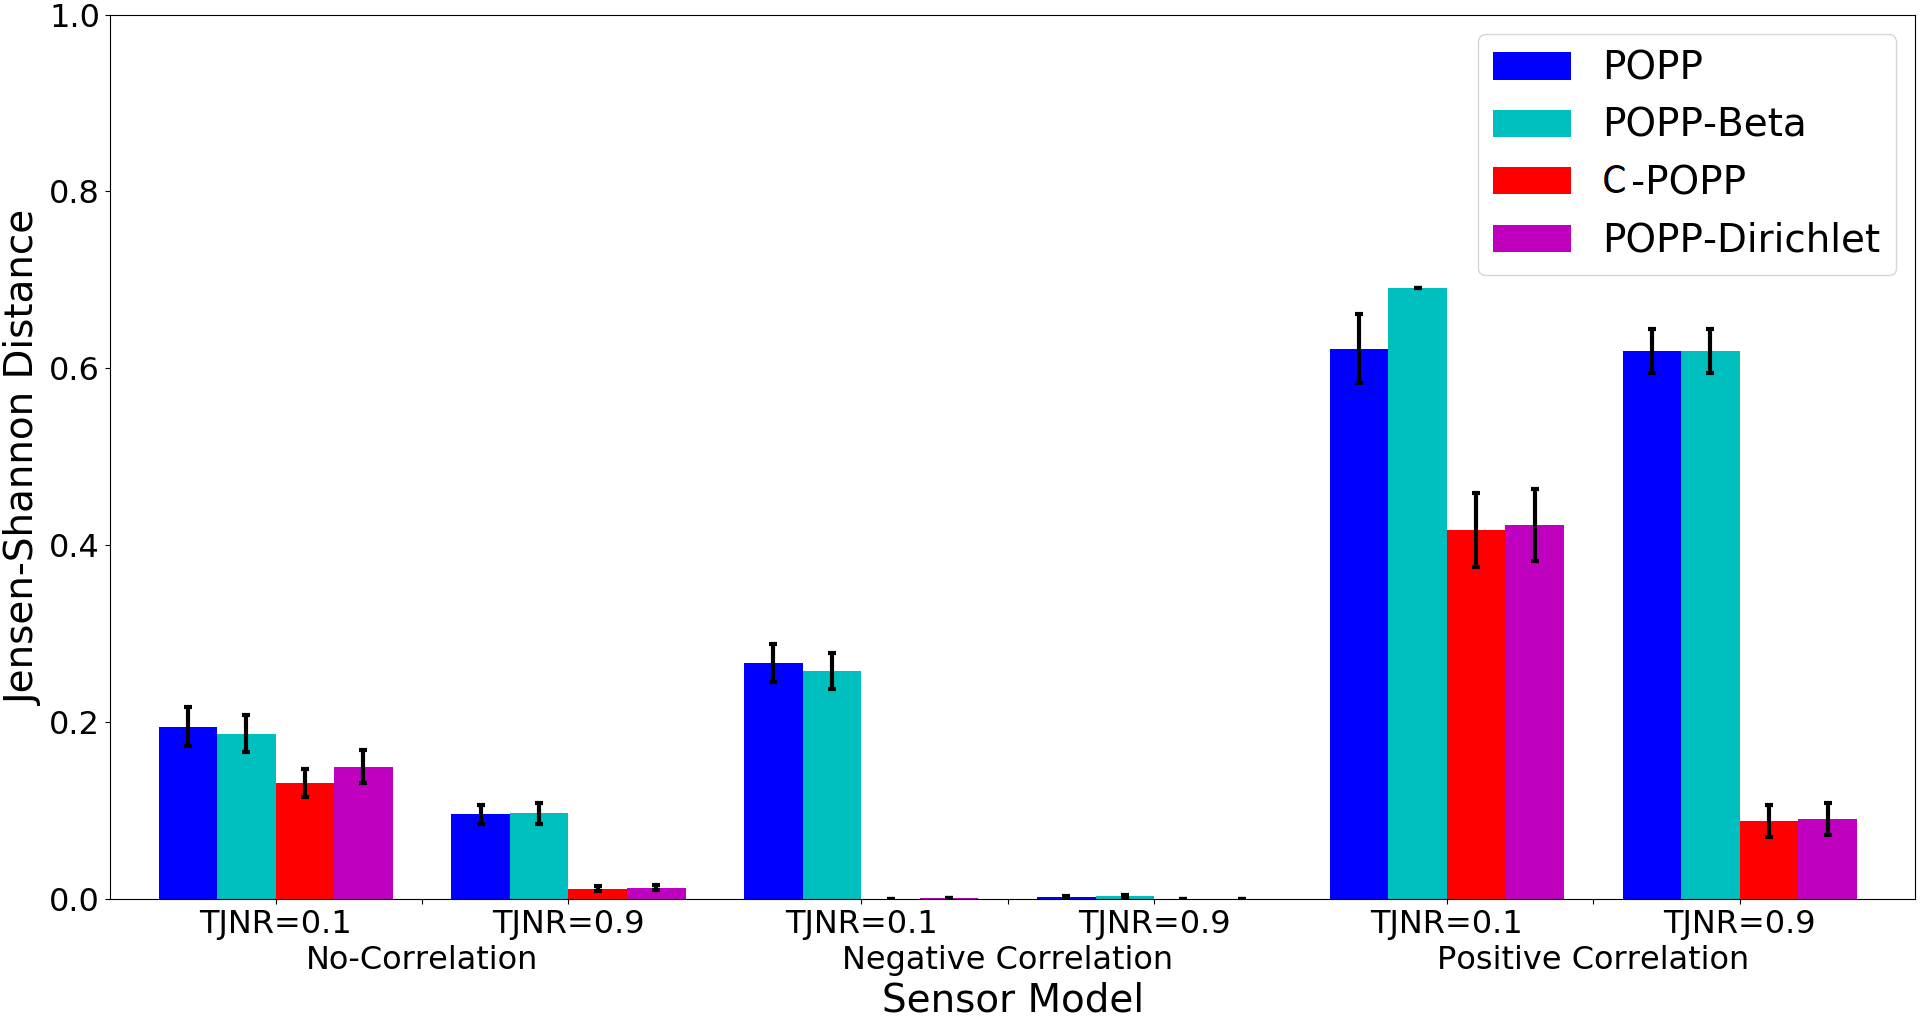
\includegraphics[width=0.5\textwidth]{./figures/tjnr_comparison_2880_kl.png}
	\caption{The Jensen-Shannon distance of posterior estimates of $\lambda$ for the POPP-Dirichlet and other POPP models with 2880 sample data used to build the (joint) sensor model with variation on $\mathcal{E^-}$. Each trial consisted of a stream of $\protect\overrightarrow{s_1} \ldots \protect\overrightarrow{s_{144}}$ samples to update $P_G(\lambda \mid \protect\overrightarrow{s_i})$. Each data point is an average of 30 trials. Standard errors are shown.} 
	\label{fig:tjnr_comparison_2880_kl}
\end{figure}
